\documentclass[aspectratio=169]{beamer}
\usepackage{ctex}
\usepackage{fontspec}

\usepackage{listings}
\usepackage{xcolor}
\usepackage{svg}

% Theme
\usetheme{Madrid}

% 使用字体必备的包
\usepackage{fontspec}

% 定义字体
\newfontfamily\noto{Noto Sans CJK SC}

% 设置beamer的字体
\setbeamerfont{normal text}{family=\noto,series=\mdseries}
\setbeamerfont{alerted text}{family=\noto,series=\bfseries}
\setbeamerfont{frametitle}{family=\noto,series=\bfseries}
% ,size={\fontsize{32}{36}}
\AtBeginDocument{\usebeamerfont{normal text}}

% Section Page
\AtBeginSection[]{
    \begin{frame}
        \vfill
        \centering
        \begin{beamercolorbox}[sep=8pt,center,shadow=true,rounded=true]{title}
            \usebeamerfont{title}\insertsectionhead\par%
        \end{beamercolorbox}
        \vfill
    \end{frame}
}

% Template
\beamertemplatenavigationsymbolsempty
\definecolor{hitszlug}{rgb}{0.145,0.203,0.758}
\definecolor{thu}{rgb}{0.50,0.36,0.71}

\setbeamercolor{section in toc}{fg=black,bg=white}
\setbeamercolor{item}{fg=hitszlug,bg=white}
\setbeamercolor{alerted text}{fg=hitszlug!80!gray}
\setbeamercolor*{palette primary}{fg=hitszlug!60!black,bg=gray!30!white}
\setbeamercolor*{palette secondary}{fg=hitszlug!70!black,bg=gray!15!white}
\setbeamercolor*{palette tertiary}{bg=hitszlug!80!black,fg=gray!10!white}
\setbeamercolor*{palette quaternary}{fg=hitszlug,bg=gray!5!white}

\setbeamercolor*{sidebar}{fg=hitszlug,bg=gray!15!white}

\setbeamercolor*{palette sidebar primary}{fg=hitszlug!10!black}
\setbeamercolor*{palette sidebar secondary}{fg=white}
\setbeamercolor*{palette sidebar tertiary}{fg=hitszlug!50!black}
\setbeamercolor*{palette sidebar quaternary}{fg=gray!10!white}

\setbeamercolor{titlelike}{parent=palette primary,fg=hitszlug}
\setbeamercolor{frametitle}{bg=gray!10!white}
\setbeamercolor{frametitle right}{bg=gray!60!white}

\setbeamercolor*{separation line}{}
\setbeamercolor*{fine separation line}{}

\setbeamertemplate{sections/subsections in toc}[square]
\setbeamertemplate{items}[square]
% Add "\usepackage{xcolor}"
% define some basic colors
\renewcommand{\lstlistingname}{code}
\definecolor{mauve}{rgb}{0.58,0,0.82}

\definecolor{codegreen}{rgb}{0,0.6,0}
\definecolor{codegray}{rgb}{0.5,0.5,0.5}
\definecolor{codepurple}{rgb}{0.58,0,0.82}
\definecolor{backcolour}{rgb}{1,1,1}



\lstset{
% listings sonderzeichen (for german weirdness)
literate={ö}{{\"o}}1
{ä}{{\"a}}1
{ü}{{\"u}}1,
basicstyle=\tiny\ttfamily,                    % very small code
breaklines=true,                              % break long lines
commentstyle=\itshape\color{green!50!black},  % comments are green
keywordstyle=[1]\color{blue!80!black},        % instructions are blue
keywordstyle=[2]\color{orange!80!black},      % sections/other directives are orange
keywordstyle=[3]\color{red!50!black},         % registers are red
stringstyle=\color{mauve},                    % strings are from the telekom
identifierstyle=\color{teal},                 % user declared addresses are teal
frame=l,                                      % black line on the left side of code
language=C,                   % all code is RISC-V
tabsize=4,                                    % indent tabs with 4 spaces
showstringspaces=false                        % do not replace spaces with weird underlines
}

\lstdefinestyle{mystyle}
{
    backgroundcolor=\color{backcolour},
    commentstyle=\color{codegreen},
    keywordstyle=\color{magenta},
    numberstyle=\tiny\color{codegray},
    stringstyle=\color{codepurple},
    basicstyle=\ttfamily\footnotesize,
    breakatwhitespace=false,
    breaklines=true,
    captionpos=b,
    keepspaces=true,
    numbers=none,
    numbersep=5pt,
    showspaces=false,
    showstringspaces=false,
    showtabs=false,
    tabsize=2,
    frame=none
}

\lstset{style=mystyle,language=C}


%Information to be included in the title page:
\title{MankorOS}
\subtitle{具有探索精神的操作系统内核开发实践展示}
\author{满洋、梁韬、苏亦凡}
\institute[HITSZ]{哈尔滨工业大学(深圳)} 
\date[\today]{ 指导老师:夏文、仇洁婷\\ \vspace{1em} \today}
\logo{
    % HITSZ logo
    
\includegraphics[height=1cm]{assets/mankoros-logo.png}
    
\includegraphics[height=1cm]{assets/hitsz.jpg}
}

\begin{document}

\frame{\titlepage}

% Sections

\section{总体介绍}

\begin{frame}
    \frametitle{Place Holder}
\end{frame}

% 我想让目录凸显我们的特殊, 所以估计只能手写了?
\begin{frame}
    \frametitle{Table of Contents}
    \tableofcontents
\end{frame}

\section{任意地址内核装载}


\begin{frame}
    \frametitle{内核装载现状观察}

    \begin{enumerate}
        \item 竞赛操作系统
              \begin{itemize}
                  \item 固定链接高位地址,汇编打开翻译
                  \item 硬编码 boot 页表到内核数据段
              \end{itemize}
        \item xv6-riscv
              \begin{itemize}
                  \item 内核使用低地址空间
                  \item 不能支持大用户程序
              \end{itemize}
        \item Linux
              \begin{itemize}
                  \item 支持装载到 \strong{任意 2M 对齐的地址} 并启动
                  \item 支持内核地址空间随机化 (KASLR)
              \end{itemize}
    \end{enumerate}

\end{frame}

\begin{frame}
    \frametitle{实现难点}

    \begin{enumerate}
        \item 不能硬编码 Boot 页表:需要 Runtime 初始化
        \item 打开翻译前内核位于低地址:需要严格位置无关代码
        \item Boot 页表的内存管理困难:内核的内存管理不可用
        \item 外设尚未初始化:没有外设,没有串口,调试困难
    \end{enumerate}

\end{frame}

\begin{frame}
    \frametitle{实现方法}

    \begin{enumerate}
        \item 汇编初始化物理 stack
        \item rust 初始化页表
              \begin{itemize}
                  \item 填充粗粒度页表 (2 MiB),使用 data 段
                  \item 映射内核映像
                  \item 映射 DTB
              \end{itemize}
        \item 返回汇编
        \item 汇编打开分页,重新初始化虚拟 stack
        \item 进入 rust main boot 流程 (SBI debug console 可用)
              \begin{itemize}
                  \item 解析 DTB
                  \item 映射设备
              \end{itemize}

    \end{enumerate}


\end{frame}

\section{设备管理}
\section{中断处理}
\section{异步协作式调度}

\begin{frame}
    \frametitle{为何采用异步设计?}

    \begin{enumerate}
        \item 底层 IO 实现是异步的
              \begin{itemize}
                  \item SD 卡 IO 可以采用中断的形式实现
                  \item 网络设备一般可用 DMA
              \end{itemize}
        \item 统一内核与用户程序的调度
              \begin{itemize}
                  \item 用户程序在执行空转操作时可以通过系统调用让出执行权, 那内核呢?
                  \item 同步内核需要手动插入调度点, 而异步内核在每一个 await 处都是调度点
              \end{itemize}
        \item Rust 提供了足够好的异步编程支持
              \begin{itemize}
                  \item 没有强制要求使用特定的运行时, 在 no-std 中也能使用
                  \item async / await 关键字提供了足够甜的语法糖
              \end{itemize}
    \end{enumerate}
\end{frame}

\begin{frame}
    \frametitle{异步内核实现要点}

    \begin{enumerate}
        \item 异步块设备与文件系统
              \begin{itemize}
                  \item 当所求数据在缓存中时, await 可以直接返回, 性能几乎与同步版本相同
                  \item 当所求数据需要从块设备中读取时, await 会主动放弃当前 CPU 执行权
              \end{itemize}
        \item 异步管道与定时任务
              \begin{itemize}
                  \item 此类任务相比起 "轮询", "通知" 显得更为自然而高效
                  \item 可以直接复用 waker 机制实现通知, 复用异步调度器实现执行, 无需额外代码
              \end{itemize}
        \item 异步睡眠锁
              \begin{itemize}
                  \item 自然地在锁竞争激烈时放弃竞争, 进入睡眠
              \end{itemize}
        \item Fallback: \texttt{loop \{ yield().await \}}
              \begin{itemize}
                  \item 该方式可以模拟一切同步内核中的写法
                  \item 不断重新加入调度器末尾 + 放弃执行权, 直到执行成功
              \end{itemize}
    \end{enumerate}
\end{frame}

\begin{frame}
    \frametitle{优势}

    在 IO 测试中 (\texttt{iozone}), 我们的内核取得了优异的成绩
    \begin{itemize}
        \item 异步实现能高效利用 CPU 执行时间, 将尽可能多的 IO 请求并行执行
        \item 相对激进的缓存策略, 尽可能填满板子的内存
    \end{itemize}

    \begin{figure}
        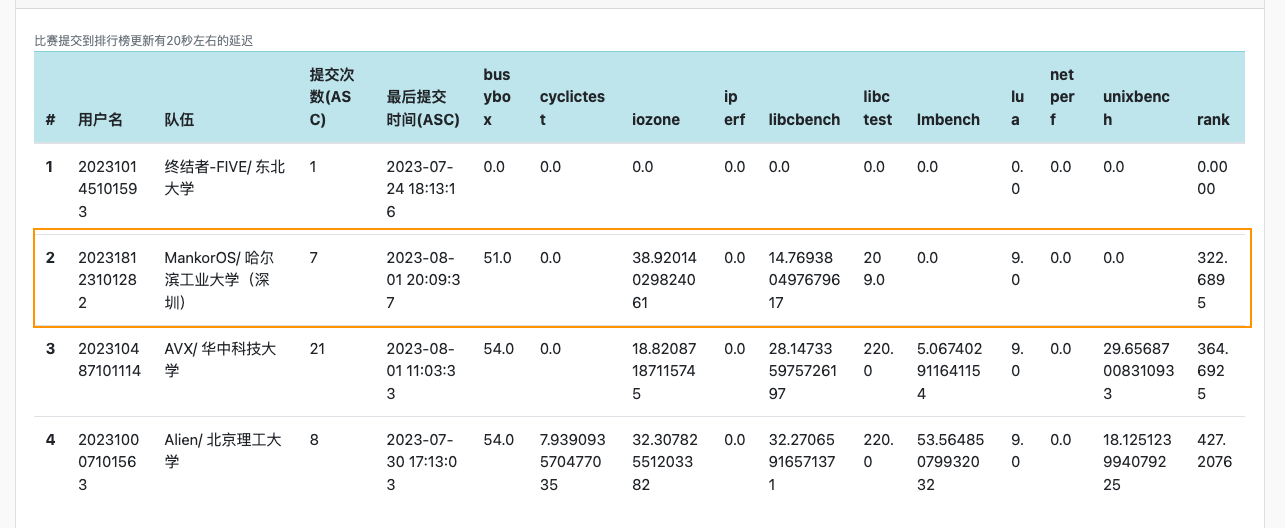
\includegraphics[width=.75\textwidth]{assets/leaderboard-final1.png}
    \end{figure}
\end{frame}

% \begin{frame}
%     \frametitle{不足}

%     \begin{enumerate}
%         \item 未能实现真正的异步 wait 系统调用
%               \begin{itemize}
%                   \item 目前仍然采用模拟同步的写法实现 wait
%                   \item 无法使得等待中的父进程 "睡熟", 性能与同步实现相比没有优势
%               \end{itemize}
%     \end{enumerate}
% \end{frame}

% 理论上这里还能加一页展望, 写写要是能突破 POSIX 限制, 异步内核能发展得怎么样
\section{特色演示}
\section{总结}

\begin{frame}
    \frametitle{开发总结}

    完成的目标:
    \begin{itemize}
        \item 同一份二进制可以在不同的硬件上启动
              \begin{itemize}
                  \item 任意地址内核装载
                  \item 基于设备树的灵活设备发现
              \end{itemize}
        \item 支持多种外设
              \begin{itemize}
                  \item 设备树解析
                  \item 能接受任意 PLIC 标准外部中断
              \end{itemize}
        \item 高性能 IO
              \begin{itemize}
                  \item 协作式调度
                  \item 多种中断处理和 DMA
              \end{itemize}
        \item 为操作系统实现细节学习提供了宝贵的资料
              \begin{itemize}
                  \item 模块化的代码
                  \item 详细的实现文档
                  \item 特殊功能的实现范例
                  \item 为 VisionFive V2 的 SD 卡驱动提供了参考实现
              \end{itemize}
    \end{itemize}

\end{frame}

\end{document}
